\documentclass[20pt]{article}
\usepackage[utf8]{inputenc}
\usepackage{amsmath, amssymb, amsthm}
\usepackage{titlesec}
\usepackage{chngcntr}
\usepackage{tikz}
\usepackage{pgfplots}
% Customization -------

% Paper size, margin
\usepackage[letterpaper,top=1.5cm,bottom=1.5cm,left=1.75cm,right=1.75cm,heightrounded]{geometry}

% line height
\renewcommand{\baselinestretch}{1.15} % line space

% Paragraph indentation 
\setlength{\parindent}{0pt} % no indent

% Paragraph spacing
\setlength{\parskip}{0.8em} % space between paragraphs

% Section number formatting
\titleformat{\section}[hang]{\bfseries}{Problem \thesection\ }{0pt}{}


% Equation numbering per section
\counterwithin*{equation}{section}
\counterwithin*{equation}{subsection}
% --------------------

\title{Problem Set 03}
\author{Farbod Mohammadzadeh\\
    1008360462}
\date{05 October 2023}

\pgfplotsset{compat = newest}

\begin{document}
\Large


\maketitle

\newpage

\section{}

\begin{align}
    h(t-\tau) = e^{2(t-\tau)} u(\tau+4-t) + e^{-2(t-\tau)} u(t-\tau - 5)
\end{align}

\begin{equation}
    e^{2(t-\tau)}u(\tau+4-t)=
    \begin{cases}
        e^{2(t-\tau)} & \text{if } \tau < t-4 \\
        0             & \text{if } \tau > t-4
    \end{cases}
\end{equation}

\begin{equation}
    e^{-2(t-\tau)}u(t-\tau - 5)=
    \begin{cases}
        e^{-2(t-\tau)} & \text{if } \tau < t+5 \\
        0              & \text{if } \tau > t+5
    \end{cases}
\end{equation}

\begin{equation}
    h(t-\tau)=
    \begin{cases}
        e^{-2(t-\tau)} & \text{if } \tau < t+5        \\
        0              & \text{if }  t-4 < \tau < t+5 \\
        e^{2(t-\tau)}  & \text{if }  t-4 < \tau       \\
    \end{cases}
\end{equation}

\[ \therefore A = t+5 \text{ and }B = t-4 \]

\section{}

\subsection*{Part a)}

\begin{equation}
    y(t)= \int_{-\infty}^{\infty} x(\tau) h(t-\tau)  \,d\tau
\end{equation}

\underline{Case 1:} No Overlap

\begin{equation}
    y(t)=0 \text{ for } t < 0 \text{ and } t - \alpha >  1 \text{ or } t  > 1 + \alpha
\end{equation}


\underline{Case 2:} Partial Overlap

\begin{equation}
    y(t)= \int_{0}^{t} x(\tau) \,d\tau  \text{ for } t \geq 0\ \& \ t - \alpha < 0 \text{ or } 0 \leq t < \alpha
\end{equation}

\underline{Case 3:} Full Overlap

\begin{equation}
    y(t)= \int_{t-\alpha}^{t} 1 \,d\tau = \alpha  \text{ for } t - \alpha \geq 0\ \& \ t < 1 \text{ or } \alpha \leq t < 1
\end{equation}

\underline{Case 4:} Partial Overlap

\begin{equation}
    y(t)= \int_{t-\alpha}^{1} 1 \,d\tau = 1 - \alpha  \text{ for } t - \alpha < 1\ \& \ t \geq 1 \text{ or } 1 \leq t <  \alpha + 1
\end{equation}

\underline{Finally:}

\begin{equation}
    y(t)=
    \begin{cases}
        t          & \text{if } 0 \leq t \leq \alpha  \\
        \alpha     & \text{if } \alpha \leq t < 1     \\
        1+\alpha-t & \text{if } 1 \leq t < 1 + \alpha \\
        0          & \text{Otherwise}                 \\
    \end{cases}
\end{equation}


\begin{center}

    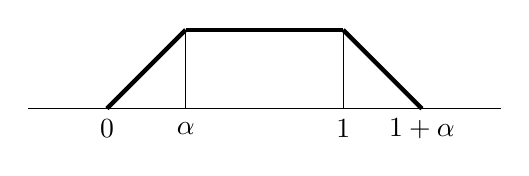
\begin{tikzpicture}[ultra thick]
        \node at (0,-0.25) {$0$};
        \draw [thin] (-1,0) -- (5,0);
        \draw (0,0) -- (1,1);
        \node at (1,-0.25) {$\alpha$};
        \draw (1,1) -- (3,1);
        \node at (3,-0.25) {$1$};
        \draw (3,1) -- (4,0);
        \node at (4,-0.25) {$1+\alpha$};

        \begin{scope}[thin]
            \draw (1,0) -- (1,1);
            \draw (3,0) -- (3,1);
        \end{scope}
    \end{tikzpicture}
\end{center}

\subsection*{Part b)}

Current discontinuities of $ \frac{dy}{d t} $ are at $ t = 0, \alpha, 1, 1 + \alpha $. To remove one of the discontinuities we can set $ \alpha = 1 $.

\section{}

\subsection*{Part a)}

\begin{eqnarray}
    y(t) &=& \int_{-\infty}^{\infty} x(\tau) h(t-\tau)  \,d\tau \\
    &=& \int_{-\infty}^{\infty} h(\tau) x(t-\tau)  \,d\tau \\
    &=& \int_{-\infty}^{\infty} h(\tau) (u(t-3-\tau) - u(t-5-\tau)) \,d\tau \\
    &=& \int_{-\infty}^{\infty} e^{-3\tau} u(\tau) (u(t-3-\tau) - u(t-5-\tau)) \,d\tau \\
    &=& \int_{0}^{\infty}  e^{-3\tau} (u(t-3-\tau) - u(t-5-\tau)) \,d\tau
\end{eqnarray}

The above $(u(t-3-\tau) - u(t-5-\tau))$ is only non-zero when $ (t-5) < \tau < (t-3) $.

\begin{eqnarray}
    y(t) &=& \int_{0}^{t-3}  e^{-3\tau} \,d\tau = \frac{1-e^{-3(t-3)}}{3}  \text{ for } 3 < t \leq 5 \\
    y(t) &=& \int_{t-5}^{t-3}  e^{-3\tau} \,d\tau = \frac{(1-e^{-5})e^{-3(t-5)}}{3}  \text{ for } t > 5
\end{eqnarray}

\begin{equation}
    \therefore y(t)=
    \begin{cases}
        0                               & \text{if } -\infty < t \leq 3 \\
        \frac{1-e^{-3(t-3)}}{3}         & \text{if } 3 < t \leq 5       \\
        \frac{(1-e^{-5})e^{-3(t-5)}}{3} & \text{if } 5 < t \leq \infty  \\
    \end{cases}
\end{equation}


\subsection*{Part b)}

\subsection*{Part c)}

\section{}

\section{}

\section{}

\section{}

\section{}

\section{}


\end{document}